\documentclass[12pt]{article}

\usepackage[margin=1in]{geometry}
\usepackage{amsmath,amssymb,amsfonts}
\usepackage{booktabs}
\usepackage{graphicx}
\usepackage{caption}
\usepackage[T1]{fontenc}
\usepackage{lmodern}
\usepackage{xcolor}
\usepackage{microtype}
\usepackage[authoryear,round]{natbib}
\usepackage{setspace}
\usepackage{tabularx}
\usepackage{pdflscape}
\usepackage{hyperref}
\hypersetup{
  colorlinks=true,
  linkcolor=blue!80!black,
  citecolor=blue!80!black,
  urlcolor=blue!80!black
}

\onehalfspacing

\title{Online Appendix: Continuous Multilevel Poisson Growth Curve Models\\
\large Supplementary Materials for ``Classifying and Predicting Degree Trajectories in Longitudinal Ego Networks''}
\author{
  Omar Lizardo\thanks{Department of Sociology, University of California, Los Angeles. Email: \texttt{olizardo@soc.ucla.edu}.}
  \and
  David Hachen\thanks{Department of Sociology, University of Notre Dame. Email: \texttt{dhachen@nd.edu}.}
}
\date{September 2026}

\begin{document}

\maketitle

\renewcommand{\thetable}{A\arabic{table}}
\renewcommand{\thefigure}{A\arabic{figure}}
\setcounter{table}{0}
\setcounter{figure}{0}

\section*{Appendix: Multilevel Growth Models}

To verify that the discrete trajectory classes identified by LCGA reflect underlying continuous growth dynamics, we estimate multilevel Generalized Linear Mixed Models (GLMMs) with a Poisson response across all eight waves:
\begin{equation}
\label{eq:glmm_full}
\log(\mathbb{E}[D_{it}]) = (\beta_0 + u_{0i}) + \beta_1 \text{Time}_{it} + \mathbf{X}_i \boldsymbol{\beta} + (\text{Time}_{it} \times \mathbf{Z}_i) \boldsymbol{\gamma}
\end{equation}
where $u_{0i} \sim \mathcal{N}(0, \sigma_u^2)$ represents random ego intercepts capturing unobserved between-person heterogeneity, $\text{Time}_{it} \in \{0, 1, \dots, 7\}$ denotes elapsed semester centered at Wave 1 baseline, $\mathbf{X}_i$ is a vector of baseline sociodemographic and personality main effects, and $\mathbf{Z}_i$ captures cross-level interactions between focal personality traits (Extraversion and Neuroticism) and elapsed time.

Table~\ref{tab:glmm_appendix} presents the model comparison fit hierarchy (Models 1--4) and the fully specified fixed effects estimates (Model 4).

\begin{table}[htbp]
\centering
\small
\caption{Fixed Effects Estimates from Multilevel Poisson Growth Curve GLMM with Random Ego Intercepts Across Eight Waves (Model 4; $N = 433$ egos, 2,456 observations)}
\label{tab:glmm_appendix}
\begin{tabularx}{\linewidth}{Xcccc}
\toprule
\textbf{Predictor Variable} & \textbf{Estimate} & \textbf{Std. Error} & \textbf{IRR [95\% CI]} & \textbf{\textit{p}-value} \\
\midrule
Intercept (Baseline Degree) & 2.53 & 0.07 & 12.55 [10.90, 14.44] & $<$ .001 \\
Time (Elapsed Waves 0--7) & -0.06 & 0.00 & 0.95 [0.94, 0.95] & $<$ .001 \\
Extraversion ($z$-score) & 0.02 & 0.02 & 1.02 [0.97, 1.07] & 0.501 \\
Neuroticism ($z$-score) & 0.01 & 0.03 & 1.01 [0.96, 1.07] & 0.609 \\
Gender Identity: Woman (ref: Man) & 0.01 & 0.04 & 1.01 [0.92, 1.10] & 0.836 \\
Race: Asian (ref: White) & -0.28 & 0.08 & 0.76 [0.65, 0.88] & $<$ .001 \\
Race: Black (ref: White) & -0.25 & 0.09 & 0.78 [0.65, 0.94] & 0.008 \\
Race: Hispanic/Latino (ref: White) & 0.02 & 0.07 & 1.02 [0.89, 1.16] & 0.773 \\
Race: Other/International (ref: White) & -0.24 & 0.09 & 0.79 [0.66, 0.95] & 0.011 \\
Parents' Income (Ordinal Scale) & 0.01 & 0.01 & 1.01 [0.99, 1.03] & 0.325 \\
Agreeableness ($z$-score) & 0.04 & 0.02 & 1.04 [0.99, 1.09] & 0.140 \\
Conscientiousness ($z$-score) & 0.00 & 0.02 & 1.00 [0.96, 1.05] & 0.965 \\
Openness ($z$-score) & -0.02 & 0.02 & 0.98 [0.94, 1.03] & 0.442 \\
Generalized Trust ($z$-score) & 0.07 & 0.02 & 1.07 [1.02, 1.12] & 0.006 \\
Time $\times$ Extraversion & -0.01 & 0.00 & 0.99 [0.99, 1.00] & 0.032 \\
Time $\times$ Neuroticism & 0.00 & 0.00 & 1.01 [1.00, 1.01] & 0.101 \\
\bottomrule
\end{tabularx}
\end{table}

Figure~\ref{fig:glmm_predicted} visualizes the predicted degree trajectories across combinations of high versus low Extraversion ($\pm 1$~SD) and high versus low Neuroticism ($\pm 1$~SD).

\begin{figure}[htbp]
\centering
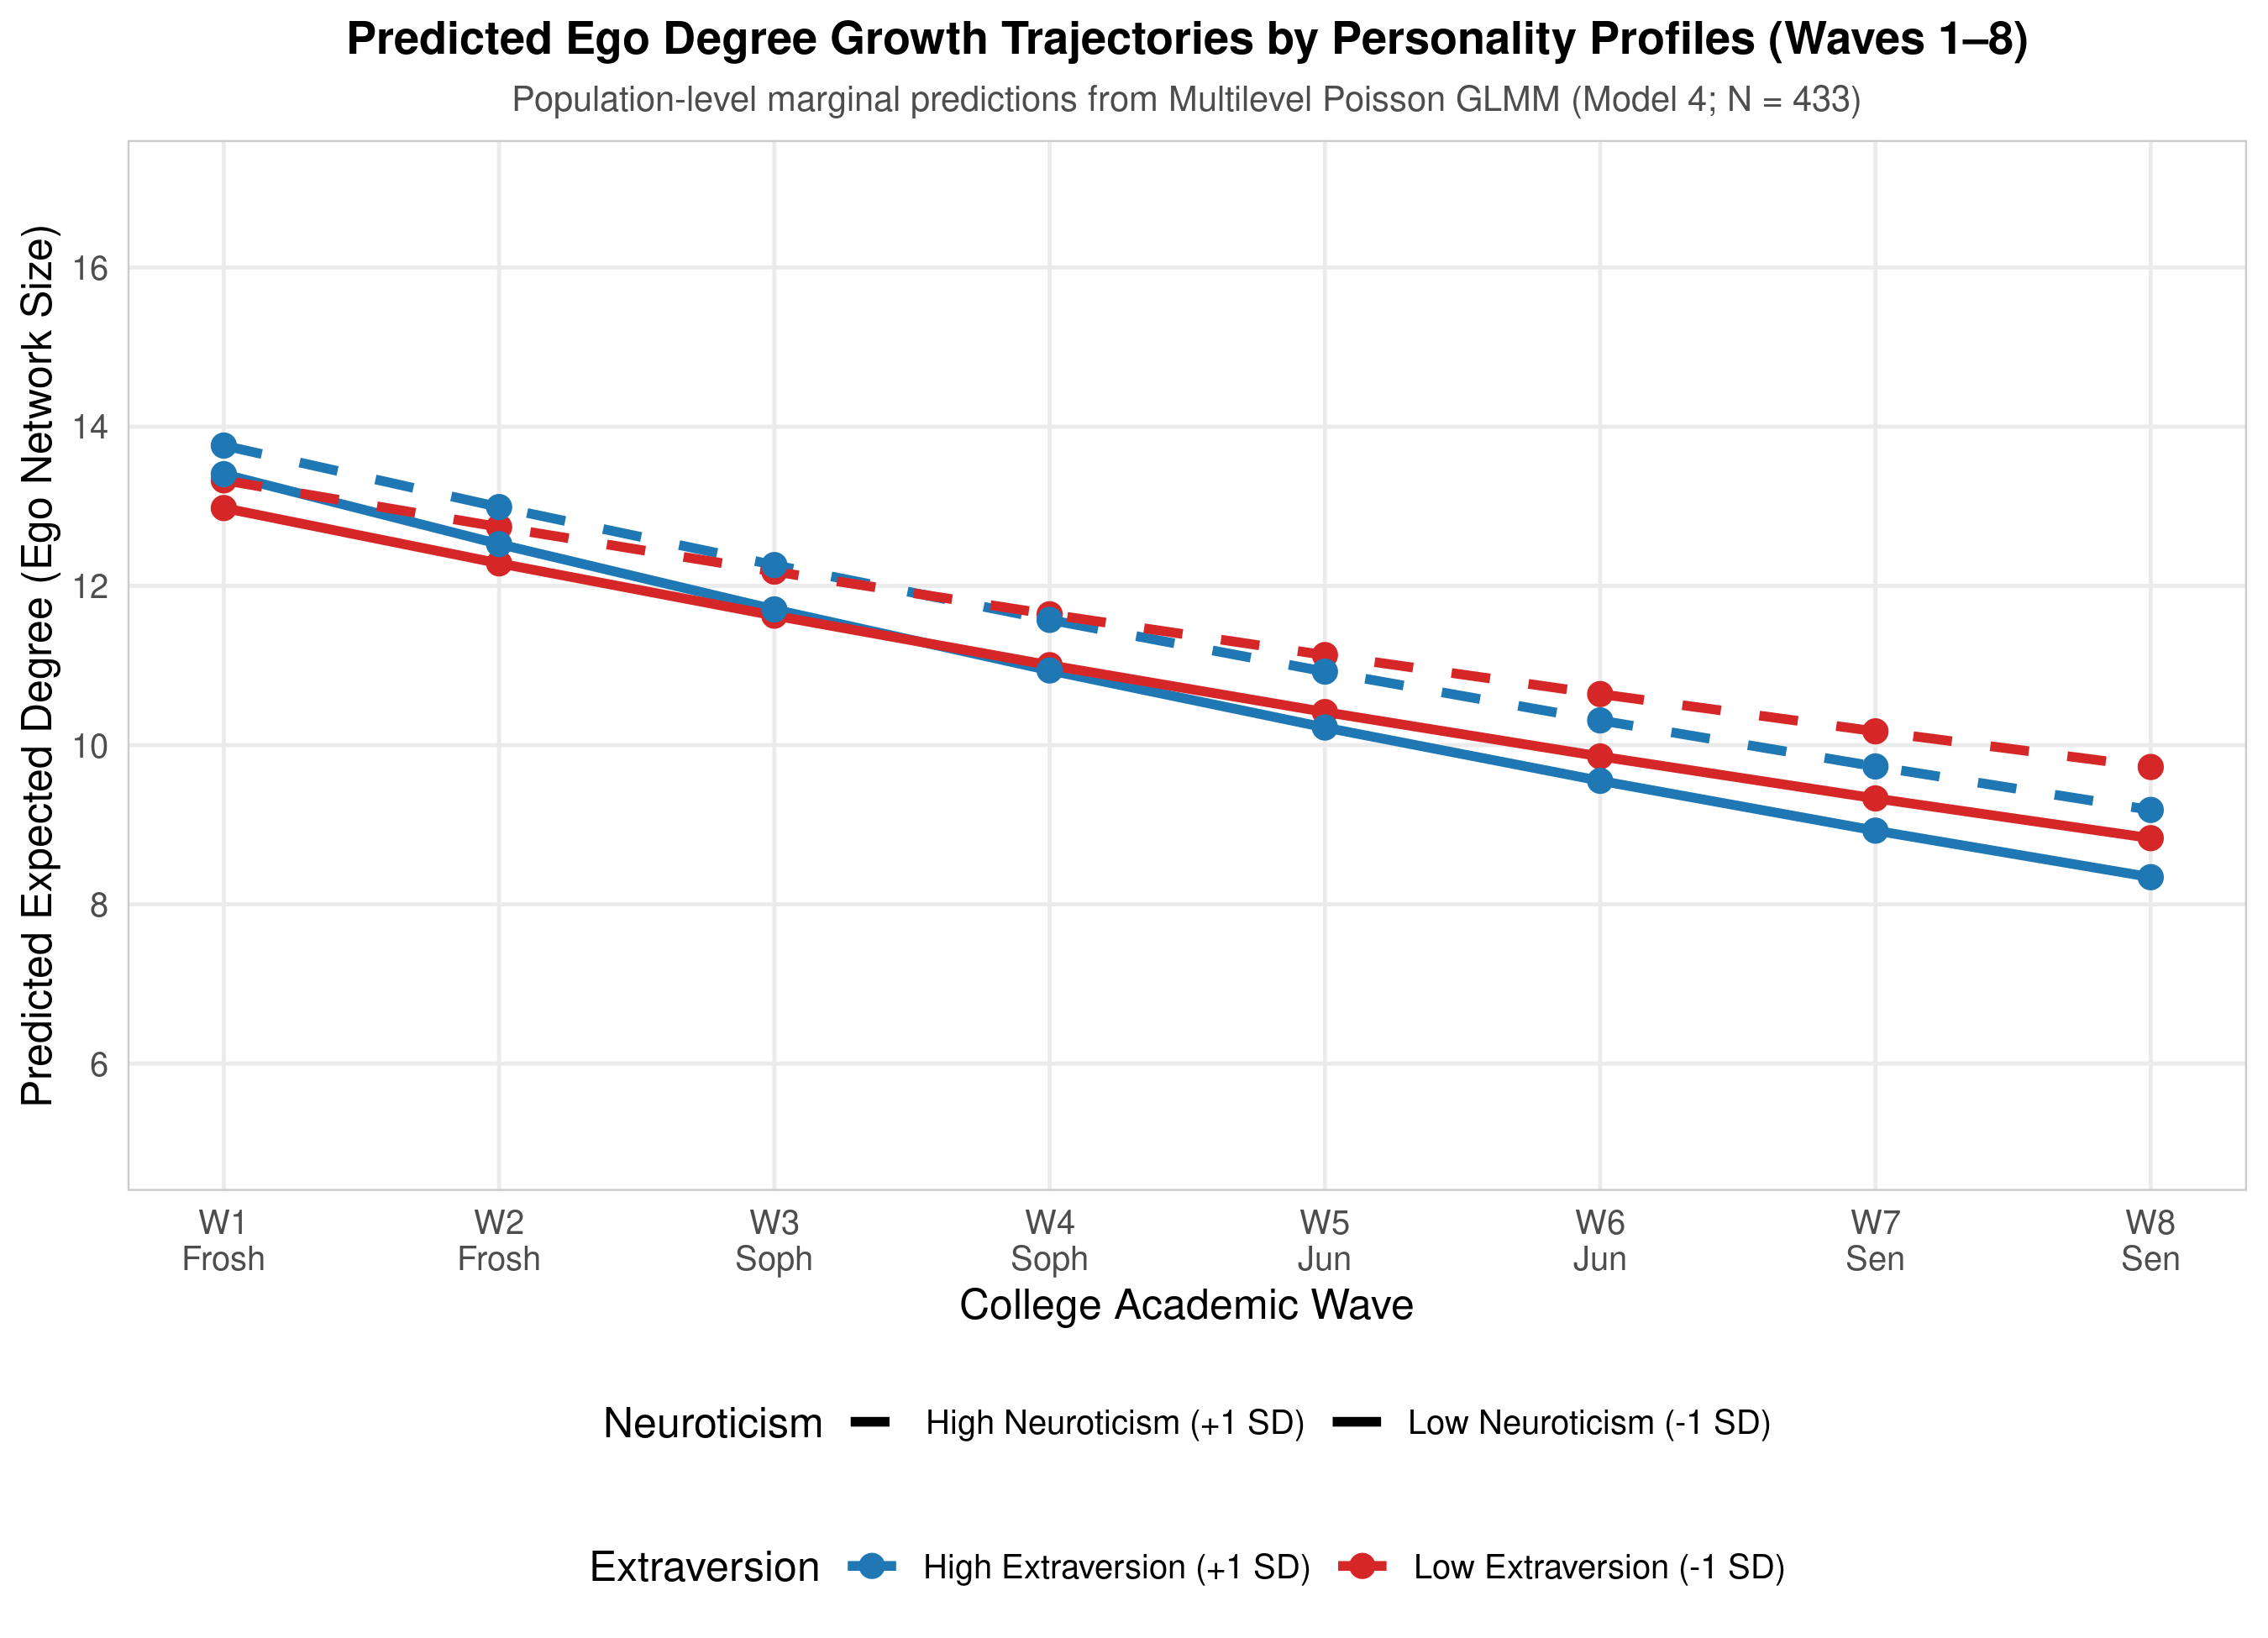
\includegraphics[width=0.85\linewidth]{Plots/figA1_multilevel_predicted_trajectories.png}
\caption{Predicted ego degree growth trajectories across eight collegiate waves by Extraversion ($\pm 1$~SD) and Neuroticism ($\pm 1$~SD) profiles estimated from Multilevel Poisson GLMM (Model 4; $N = 433$).}
\label{fig:glmm_predicted}
\end{figure}

The continuous growth estimates directly corroborate our primary mixture findings. On average, student ego networks contract by 5.5\% per elapsed collegiate wave ($\text{IRR} = 0.945, p < 0.001$). Baseline Generalized Trust exerts a significant positive main effect on network scale ($\text{IRR} = 1.071, p = 0.006$), confirming that trusting students sustain larger personal communities throughout college. Furthermore, the interaction between Time and Extraversion is statistically significant and negative ($\text{IRR} = 0.994, p = 0.032$). As shown in Figure~\ref{fig:glmm_predicted}, extraverted students enter college with larger initial networks ($\approx 13.4$--13.8 alters at Wave 1 vs.~$\approx 12.9$--13.3 for introverts) but undergo a faster rate of winnowing, crossing below their introverted peers by senior year ($\approx 8.3$--9.2 alters vs.~$\approx 8.8$--9.7 alters).

\clearpage
\bibliographystyle{apalike}
\bibliography{references}

\end{document}
